\documentclass[12pt,oneside,a4paper,parskip]{scrbook}
\usepackage[utf8]{inputenc}
\usepackage{csquotes}
\usepackage[ngerman]{babel}
\usepackage{floatflt}
\usepackage{subfigure}
\usepackage[pdftex]{graphicx}
\graphicspath{ {./pictures/} }
\usepackage[hidelinks]{hyperref}
\usepackage{color}
\usepackage{amssymb}
\usepackage{textcomp}
\usepackage{nicefrac}
\usepackage{scrhack}
\usepackage{pdfpages}
\usepackage{float}
\usepackage{pdflscape}
\usepackage{subfigure}
\usepackage{pdfpages}
\usepackage[verbose]{placeins}
\usepackage[nouppercase,headsepline,plainfootsepline]{scrlayer-scrpage}
\usepackage{listings}
\usepackage{xcolor}
\usepackage{color}
\usepackage{caption}
\usepackage{subfigure}
\usepackage{epstopdf}
\usepackage{longtable}
\usepackage{setspace}
\usepackage{booktabs}
\usepackage[style=numeric,backend=biber]{biblatex}
\bibliography{./thesis.bib}



%%%%%%%%%%%%%%%%%%%
%% definitions
%%%%%%%%%%%%%%%%%%%
\def\BaAuthor{Lennard Rose, Jochen Schmidt, Moritz Zeitler}
\def\BaAuthorStudyProgram{Informatik} %% Wirtschaftsinformatik, E-Commerce, Informationssysteme
\def\BaType{Projektarbeit} %% Masterarbeit
\def\BaTitle{Entwicklung einer Data Mining Plattform f\"ur Corona Daten}
\def\BaSupervisorOne{Prof. Rott}
\def\BaSupervisorTwo{Prof. Fertig}
\def\BaDeadline{\today}

\ifdefined\iswithfullname
  \def\ShowBaAuthor{\BaAuthor}
\else
  \def\ShowBaAuthor{N.~N.}
\fi

\hypersetup{
pdfauthor={\ShowBaAuthor},
pdftitle={\BaTitle},
pdfsubject={Subject},
pdfkeywords={Keywords}
}

%%%%%%%%%%%%%%%%%%%
%% configs to include
%%%%%%%%%%%%%%%%%%%
\colorlet{punct}{red!60!black}
\definecolor{background}{HTML}{EEEEEE}
\definecolor{delim}{RGB}{20,105,176}
\colorlet{numb}{magenta!60!black}

\definecolor{gray}{rgb}{0.4,0.4,0.4}
\definecolor{darkblue}{rgb}{0.0,0.0,0.6}
\definecolor{cyan}{rgb}{0.0,0.6,0.6}

\definecolor{pblue}{rgb}{0.13,0.13,1}
\definecolor{pgreen}{rgb}{0,0.5,0}
\definecolor{pred}{rgb}{0.9,0,0}
\definecolor{pgrey}{rgb}{0.46,0.45,0.48}

\lstset{
  basicstyle=\ttfamily,
  columns=fullflexible,
  showstringspaces=false,
  commentstyle=\color{gray}\upshape
  linewidth=\textwidth
}

\lstdefinelanguage{json}{
    basicstyle=\normalfont\ttfamily,
    numbers=left,
    numberstyle=\scriptsize,
    stepnumber=1,
    numbersep=8pt,
    showstringspaces=false,
    breaklines=true,
    backgroundcolor=\color{background},
    literate=
     *{0}{{{\color{numb}0}}}{1}
      {1}{{{\color{numb}1}}}{1}
      {2}{{{\color{numb}2}}}{1}
      {3}{{{\color{numb}3}}}{1}
      {4}{{{\color{numb}4}}}{1}
      {5}{{{\color{numb}5}}}{1}
      {6}{{{\color{numb}6}}}{1}
      {7}{{{\color{numb}7}}}{1}
      {8}{{{\color{numb}8}}}{1}
      {9}{{{\color{numb}9}}}{1}
      {:}{{{\color{punct}{:}}}}{1}
      {,}{{{\color{punct}{,}}}}{1}
      {\{}{{{\color{delim}{\{}}}}{1}
      {\}}{{{\color{delim}{\}}}}}{1}
      {[}{{{\color{delim}{[}}}}{1}
      {]}{{{\color{delim}{]}}}}{1},
}

\lstset{language=xml,
  morestring=[b]",
  morestring=[s]{>}{<},
  morecomment=[s]{<?}{?>},
  stringstyle=\color{black},
  numbers=left,
  numberstyle=\scriptsize,
  stepnumber=1,
  numbersep=8pt,
  identifierstyle=\color{darkblue},
  keywordstyle=\color{cyan},
  backgroundcolor=\color{background},
  morekeywords={xmlns,version,type}% list your attributes here
}

\lstset{language=Java,
  showspaces=false,
  showtabs=false,
  tabsize=4,
  breaklines=true,
  keepspaces=true,
  numbers=left,
  numberstyle=\scriptsize,
  stepnumber=1,
  numbersep=8pt,
  showstringspaces=false,
  breakatwhitespace=true,
  commentstyle=\color{pgreen},
  keywordstyle=\color{pblue},
  stringstyle=\color{pred},
  basicstyle=\ttfamily,
  backgroundcolor=\color{background},
%  moredelim=[il][\textcolor{pgrey}]{$$},
%  moredelim=[is][\textcolor{pgrey}]{\%\%}{\%\%}
}

\newcommand*{\forcetwosidetitle}[1][1]{%
 \begingroup
   \cleardoubleoddpage
   \KOMAoptions{titlepage=true}% useful e.g. for scrartcl
   \csname @twosidetrue\endcsname
   \maketitle[{#1}]
 \endgroup
}


\begin{document}


%%%%%%%%%%%%%%%%%%%
%% Titelseite
%%%%%%%%%%%%%%%%%%%


\frontmatter
\titlehead{%  {\centering Seitenkopf}
  {Hochschule für angewandte Wissenschaften Würzburg-Schweinfurt\\
   Fakultät Informatik und Wirtschaftsinformatik}}
\subject{\BaType}
\title{\BaTitle\\[15mm]}
\subtitle{\normalsize{vorgelegt an der Hochschule f\"{u}r angewandte Wissenschaften W\"{u}rzburg-Schweinfurt in der Fakult\"{a}t Informatik und Wirtschaftsinformatik zum Abschluss eines Studiums im Studiengang \BaAuthorStudyProgram}}
\author{\ShowBaAuthor}
\date{\normalsize{Eingereicht am: \BaDeadline}}
\publishers{\
  \normalsize{Erstpr\"{u}fer: \BaSupervisorOne}\\
  \normalsize{Zweitpr\"{u}fer: \BaSupervisorTwo}\\
}
\forcetwosidetitle


%%%%%%%%%%%%%%%%%%%
%% abstract
%%%%%%%%%%%%%%%%%%%

\section*{Zusammenfassung}

TODO

\section*{Abstract}

TODO

\newpage
\chapter*{Danksagung}



%%%%%%%%%%%%%%%%%%%
%% Inhaltsverzeichnis
%%%%%%%%%%%%%%%%%%%
\tableofcontents



%%%%%%%%%%%%%%%%%%%
%% Main part of the thesis
%%%%%%%%%%%%%%%%%%%
\mainmatter

\chapter{Einführung und Motivation}\label{ch:intro}
Wir in unserem Team, bestehend aus Jochen Schmidt, Lennard Rose und Moritz Zeitler hatten nach unserem Gemeinsamen Programmierprojekt beschlossen, wieder zusammen zu arbeiten und diesmal in eine ganz andere Richtung zu gehen. Hierzu muss man wissen, dass unser Programmierprojekt damals aus einem Multiplayer-Computerspiel bestand, welches wir ausschließlich mit C++ sowie SDL programmierten. Da wir nichts vorgefertigtes an Code oder Lösungen benutzten und alles \"von der Pike auf\" entwickelten, lag der Fokus vor allem auf Algorithmen, Datenstrukturen und Patterns. Auch wenn uns diese Art des Entwickelns allen sehr Spaß gemacht hat und unser Projekt sehr Erfolgreich war, wollten wir mit dieser Projektarbeit nochmal in eine ganz andere Richtung gehen um uns als Entwickler weiter zu entwickeln und unserem Toolset ein paar neue XY hinzuzufügen. Mit dem Thema Datamining war für uns auch sehr schnell ein Thema gefunden, Coronadaten boten sich aus aktuellem Anlass an und da Moritz noch ein paar alte Rechner im Keller stehen hatte, beschlossen wir nicht nur eine Lösung, sondern ein betriebsbereites System zu entwickeln. \newline


\chapter{Cluster}
Grunds\"atzlich wird das komplette Projekt auf Basis eines Hadoop Cluster erstellt. Hadoop ist ein Framework f\"ur die skalierbare und verteilt arbeitende Software. Gerne wird auch der Begriff  Hadoop \"Okosystem verwendet da es einen kompletten Zoo von Technologien (z.B. Zookeeper, HBase, Flink, Storm, Pig, Solr) gibt die im Hadoop Umfeld verwendet werden kann. Hadoop erm\"oglicht eine horizontale Skalierung, dies bedeutet das dem System dynamisch zus\"atzliche Knoten, angeh\"angt werden k\"onnen die dann die Rechenleistung, bzw die Speicherkapazit\"at des Clusters erh\"ohen. In der Basis besteht Hadoop aus YARN und dem HDFS die zusammen mit dem MapReduce Konzept eine Datenverarbeitung erm\"oglichen. Zus\"atzlich zu diesen Standardkomponenten wurden noch Apache Oozie sowie Apache Zeppelin installiert. Diese einzelnen Konzepte sowie zus\"atzliche Basisinformationen zum Cluster werden im folgenden noch genauer erkl\"art.
\section{YARN}
YARN steht f\"ur 'Yet another resource negotiater'. Die Aufgabe des YARN darin die verf\"ugbaren Ressourcen auf alle anfallenden Aufgaben zu verteilen. Dies bedeutet YARN ist 'Resourcemanager' als auch 'Job-Scheduler'.
\begin{figure}[H]
	\centering
	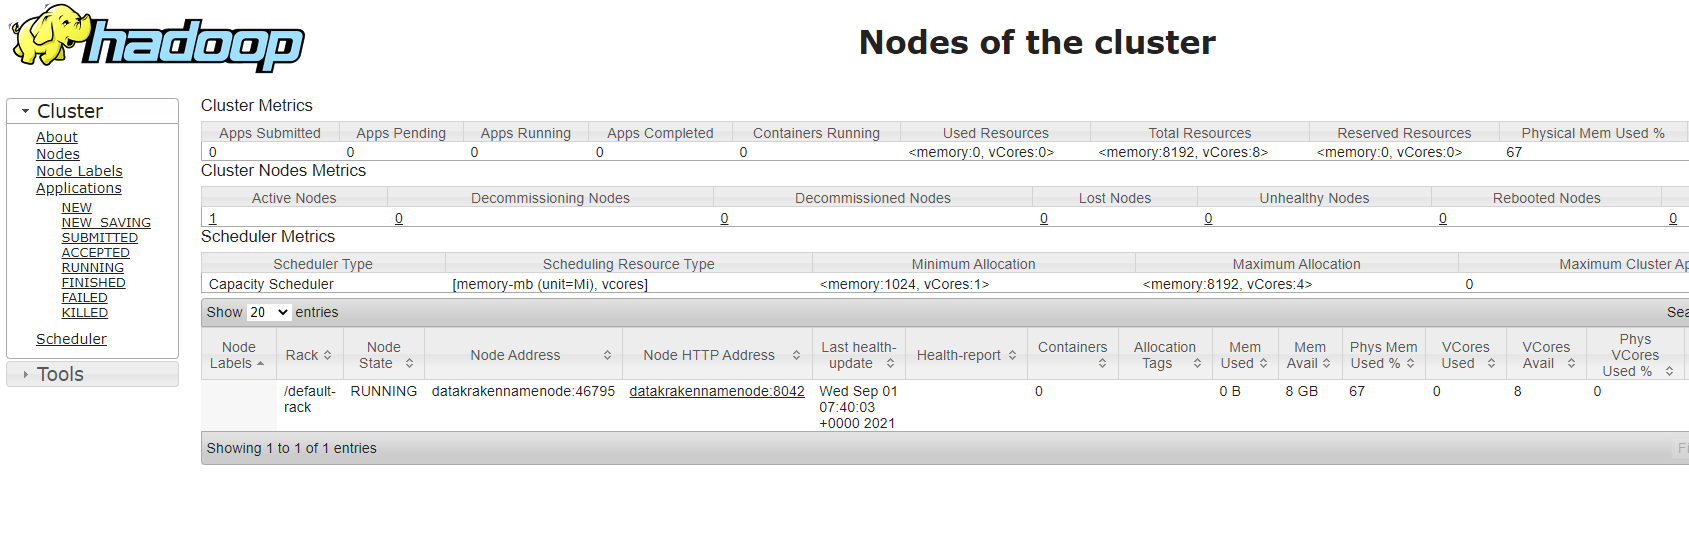
\includegraphics[scale=0.3]{yarnClusterOverview.png}
	\captionsetup{justification=centering}
	\caption{\"Ubersichtsseite von YARN}
	\label{pic:yarnClusterOverview}
\end{figure}
Bevor YARN zu seinem Namen kam wurde der Dienst zun\"achst 'MapReduce2' genannt. Jedoch entwickelte sich YARN dann schnell dahingehend das auch noch andere Aufgaben neben MapReduce, wie zum Beispiel interaktive Abfragen oder Echtzeit-Analysen von Streaming-Daten, ausgef\"uhrt werden k\"onnen, was dazuf\"uhrte die Verbindung zu MapReduce im Namen aufzul\"osen. \newline
Die tats\"achliche grundlegende Idee hinter der Funktion von YARN ist das Aufspalten von 'ResourceManager' und 'ApplicationMaster'. Der ResourceManager ist die zentrale Komponente mit dem der User in Kommunikation steht oder besser gesagt mit dem eine Anfrage an Rechenkapazit\"at kommuniziert. F\"ur eine solche Anfrage erstellt der 'ResourceManager' einen enstprechenden 'ApplicationMaster', dieser k\"ummert sich dann von Anfang bis Ende um diesen einen Auftrag. Status, Neustart oder Fehlerbehandlung werden komplett von ihm \"ubernommen der 'ResourceManager' hat damit nichts mehr zu tun. Der 'ApplicationMaster' \"ubergibt seine Aufgabe an einen Nodemanager der dann die tatsa\"achliche Ausf\"uhrung startet, bzw eine Container entgegen nimmt und diesen ausf\"uhrt. Die \"Uberwachung dieses Containers ist allerdings wiederum, wie bereits erw\"ahnt, Aufgabe des 'ApplicationMaster'. Nach Abschluss der Ausf\"uhrung meldet sich der 'ApplicationMaster' wieder beim 'ResourceManager' ab und gibt seine Ressourcen wieder frei.\cite{Shenoy.2014}
\begin{figure}[H]
	\centering
	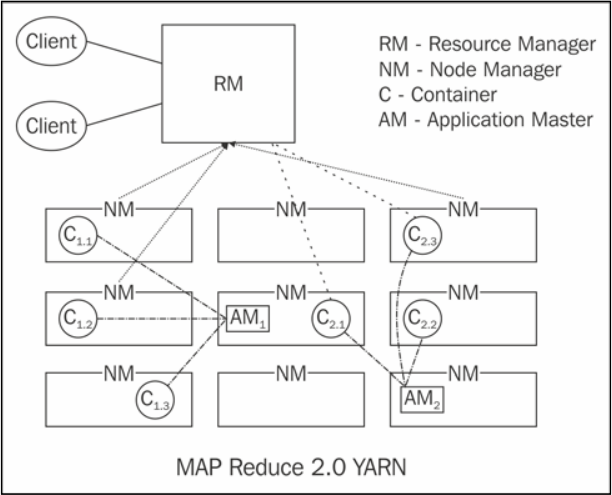
\includegraphics[scale=0.9]{yarnOverview.png}
	\captionsetup{justification=centering}
	\caption{Visualisierung der Aus\"uhrung eines YARN-Containers}
	\label{pic:yarnOverview}
\end{figure}
Dies ist an dieser Stelle wahrscheinlich durchaus unverst\"andlich, was allerdings f\"ur den nachfolgenden Bericht nicht all zu relevant ist.
\newline An dieser Stelle ist es wichtig zu erw\"ahnen das die Auftr\"age die von YARN ausgef\"uhrt werden immer in Containern ausgef\"uhrt werden, vergleichbar mit Docker oder Kubernetes. Dies bedeutet das alle Abh\"angigkeiten mit in den Container geliefert werden m\"ussen. Außerdem ist zu beachten das es teilweise zu Problemen mit Netzwerk bzw. Internetzugriff kommen kann.
\section{HDFS}
Das 'Hadoop Distributed File System' ist die Technologie, die im Hadoop Umfeld die verteilte Datenablage erm\"oglicht. HDFS hat viele Gemeinsamkeiten zu andern bekannten verteilten Dateisystemen wie zum Beispiel Amazon S3. Der Hauptunterschied zu den meisten Technologien ist Widerstandsf\"ahigkeit gegen\"uber Fehlern. Der Grundsatz von Hadoop war immer das ein Cluster aus Standard bzw. Kosteng\"unstiger Hardware aufgebaut werden kann, was allerdings zu einer h\"ohren Fehleranf\"alligkeit f\"uhren kann. Das HDFS wurde in diesem Zusammenhang nach dem Grundsatz entwickelt das es immer ein Teil der Hardware nicht funktioniert.\cite{hdfsFailure} \newline
Mit unter der wichtigste Grundsatz ist aber wahrscheinlich dass, wenn m\"oglich, nicht die Daten zum Prozess bewegt werden sondern der Code bzw. der Algorithmus zu den Daten gebracht wird.\cite{movingComputation} Je gr\"osser der Datensatz desto gr\"osser die Kosten diese Daten zu verschieben. Und da sich im Normalfall ein 'BigData' System haupts\"achlich um grosse Datenmengen k\"ummert wird dieser Prozess genau umgedreht, der Algorithmus kommt zu den Daten. Die n\"otigen Voraussetzungen und Schnittstellen stellt das HDFS zur Verf\"ugung um Applikationen es zu erm\"oglichen diese Idee umzusetzen.
\section{Oozie und Cron}
\section{Zeppelin}

\chapter{Entwicklungsprozess}
Beim Entwicklungsprozess wurde sich f\"ur eine Scrum artige L\"osung entschieden. So werden klassische Artefakte und Tools wie etwa das Daily oder der Backlog entsprechend angepasst angewandt. Anpassung meist im Sinne der zeitlichen Komponente. Da das Projekt parallel w\"ahrend des Semesters abl\"auft wurde hier das 'Daily', von einem t\"aglichen auf einen w\"ochentlichen Rhythmus umgestellt. Das Backlog wird durch das Team selbst bef\"ullt da es keinen 'Product Owner' gibt. Genauso wurden die Sprints abgewandelt, durch die zeitliche Entzerrung wird hier direkt auf eine dynamische Sprintl\"ange gesetzt die jeweils zum Sprint-Anfang abgestimmt worden ist. \newline
G\"anzlich verzichtet wurde auf die Sprint Retrospektive, zwar hat sich im Laufe des Projekts der Prozess dynamisch angepasst, allerdings wurde hier nicht explizit ein Artefakt bzw. Termin durchgef\"uhrt. \"Anderungen am Prozess wurden kurzfristig und in direkter Absprache mit allen Teammitgliedern beschlossen.


\chapter{Datenablagekonzept}
F\"ur die Datenablage wurde zun\"achst ein entsprechendes Konzept entwickelt. Dieses Konzept basiert auf den Daten die abgelegt werden sollen. Hierzu wird zun\"achst ein \"Uberblick \"uber die zu ablegenden Daten gegeben:
\begin{itemize}
	\item Corona Nachrichten/Artikel
	\item Corona RKI Daten
	\item Corona Maßnahmen
	\item Wetterdaten
\end{itemize}
Jede einzelne Datenquelle wird nun genauer beleuchtet und ein entsprechendes Datenablagekonzept erarbeitet. Da die Konzepte sich aber sehr \"ahneln wird der Hauptteil der Erkl\"arung bei der gr\"ossten Komponente den Corona-Artikeln zu finden sein. Grunds\"atzlich werden alle Daten sowohl in Elasticsearch als auch im HDFS abgelegt. Wobei das HDFS haupts\"achlich f\"ur Data Governance Zwecke genutzt wird. Bedeutet das hier die Rohdaten unver\"andert gespeichert werden sollen um sp\"ater immer noch Zugriff auf die Original Daten zu haben, was eine Art 'sanity-check' der Daten erm\"oglicht.
\section{Corona Nachrichten/Artikel}
Die Corona Nachrichten bzw. Artikel werden in zwei unterschiedlichen Technologien abgelegt. Zun\"achst betrachten wir die Rohdaten. Wie bereits erkl\"art wird jeder Artikel in Rohformat gespeichert. Diese Daten sind aber f\"ur die Auswertung und zur \"Ubersicht der Datensammlung erst mal unwichtig. Dies bedeutet das diese Daten nicht in einer Datenbank indiziert, sondern nur im HDFS abgelegt werden. Die Geschwindigkeit des HDFS f\"ur den Datenzugriff ist ausreichend um die Daten bei einer genauen Auswertung ad-hoc zu lesen. Streng genommen k\"onnte man sogar argumentieren dass das HDFS nichts anderes als ein 'key-value store' ist. So wird im Hintergrund eine Datei die unter einem gewissen Pfad abgelegt worden ist f\"ur den User als klassischer Dateipfad angezeigt (Ordner durch 'forward-slashes' getrennt und am Ende des Pfades ein Dateiname), intern aber der Pfad einen key darstellt. Dies ist n\"otig um die Verteilung und Ausfallsicherheit der Daten \"uber mehrere Knoten gew\"ahrleisten zu k\"onnen. Allerdings ist dies f\"ur den User faktisch nicht bemerkbar, da dieser immer mit den entsprechenden Pfaden arbeitet.
Um nun den Kreis zu schliessen werden nicht nur Meta-Daten der Artikel gespeichert sondern auch der komplette Artikel im Rohformat um Datenverlust vorzubeugen und die Konsistenz der Daten sp\"ater noch pr\"ufen zu k\"onnen. Die Rohdaten werden dann abgelegt unter dem Pfad: '/datakraken/articles/\$bundesland\$/\$Zeitung\$/\$Datum\$/\$ArtikelId\$\_\$TimeStamp\$'. Dieser Pfad wird dann zu den Meta-Daten hinzugef\"ugt.
Nun zu den Meta-Daten, diese kommen werden vom entsprechenden Scraper erzeugt. Dies Daten werden dann im Elasticsearch Cluster abgelegt unter entsprechendem Index Namen. Dies hilft dabei eine \"Ubersicht zu den Daten zu erhalte, einen Status zu bekommen in welchem Mass die Daten in das System kommen und erm\"oglicht eine rudiment\"are Analyse. Die Daten an sich sind definiert durch die entsprechende Config
\section{Corona RKI Daten}
Die wichtigsten Basis Informationen \"uber den Status der Corona-Pandemie in Deutschland sind h\"ochst wahrscheinlich Inzidenz-Wert und Impfquote. Diese Informationen werden in diesem Projekt \"uber das Robert-Koch-Institut bezogen. \"Uber eine \"offentliche API kann nicht nur Inzidenzwert pro Bundesland, sondern auch per Bezirk bezogen werden. Ausserdem sind alle Informationen zum derzeitigen Impfstand in Deutschland, sowie Informationen zu PCR- und Schnelltests in Deutschland verf\"ugbar. Alle Informationen die hier von der API zur Verf\"ugung gestellt werden, werden auch gespeichert. Hier folgt der Scraper dem Allgemeinen Konzept, die Original Daten werden im HDFS abgelegt und dann mit minimaler Ver\"anderung im Elasticsearch indiziert.
\section{Corona Maßnahmen}
Das soeben erw\"ahnte Konzept der Nachrichten wird genauso f\"ur die Massnahmen verwendet. Rohdaten werden im HDFS abgelegt, w\"ahrend die beschreibenden Daten im Elasticsearch indiziert werden. Diese Massnahmen werden mit folgendem Pattern abgelegt: '/datakraken/measures/\$bundesland\$/\$Zeitung\$/\$Datum\$/\$ArtikelId\$\_\$TimeStamp\$'.
\section{Corona Basis Daten}
\section{Wetterdaten}
Auch die Wetterdaten werden im gleichen Stil abgelegt. Heisst die einzelnen Wetterlogs werden als Dokumente im Elasticsearch abgelegt und auch hier\"uber abgefragt. Allerdings werden die Wetterdaten auch noch entsprechend des allgmeinen Konzepts im HDFS abgelegt. Die Ablage Struktur im HDFS ist in folgendem Pattern:  '/datakraken/weather/\$Stadt\$/\$Datum\$/\$TimeStamp\$'.
\section{'Querdenker' Telegram Gruppen}
Im Bereich der Telegram Gruppen muss hier differenziert werden. Die verschickten Nachrichten an sich werden mit den Meta-Daten zusammen im Elasticsearch abgelegt. H\"angt allerdings an der Nachricht noch eine Datei ein, oder ein Link, wird die Datei im HDFS abgelegt. Dazu wird eine Referenz erstellt und mit im Elasticsearch abgelegt. Die Ablage Struktur im HDFS ist in folgendem Pattern: '/datakraken/telegram/\$GruppenName\$/\$Datum\$/\$NachrichtId\$\_\$TimeStamp\$'.

\chapter{Cluster und Deployment}
%mehr so braindump, überarbeiten%
\section{Überblick} Bereits bei der Ideenfindung zu unserer Projektarbeit hatten wir uns dazu entschieden, nicht nur den Quellcode für den Datensammler zu schreiben, sondern das ganze auch auf einem Cluster zum laufen zu bringen. Hierfür haben wir 3 alte Rechner (Bis zur explosion eines Netzteils ursprünglich 4) von Moritz genommen. Die Absicht hier war, aus alter, ungenutzter Hardware, neuen Wert zu schöpfen. Tieferen Einblick in Serververwaltung erhalten. Bla bla weitere gründe ausdenken. Wir haben bewusst von der Verwendung von Docker abgesehen, trotz des Wissens, dass es die einfachste Möglichkeit wäre die Software auf dem Cluster zu deployen. Grund ist, dass wir dieses Projekt vornehmlich dazu nutzen wollen, ein breites Fundament an Wissen aufzubauen, welches auch Serveradministration beinhalten soll. Um Elasticsearch mit Docker zu starten, ist nicht viel mehr nötig als sich ein Compose-File aus dem Internet zu suchen und zu starten. Retrospektiv betrachtet hat sich diese Erwartung erfüllt und durch das troubleshooting

\section{Betriebssystem} Als Betriebssystem wählten wir Ubuntu 18.04 LTS, da es mit ca. einem Drittel aller Linuxserver das meistverwendete Betriebssystem darstellt. Als Bezeichnung für die einzelnen Knoten wählten wir "datakrakennamenode", für den Masternode, sowie "datanodekraken1" und "datanodekraken2", für die beiden Anderen. Auf jedem Knoten legten wir einen User mit Namen "Hadoop" an. Im laufe des Projekts stellte sich heraus, dass eine "sauberere" Lösung gewesen wäre, einen User zu allgemeinen Serververwaltung, sowie jeweils einen User zum laufen der Elasticsearch sowie Hadoop Daemons zu erstellen. Auch wurde der Fehler gemacht den Rootuser nur Stiefmütterlich zu behandeln und nicht mit Passwort einzurichten, dies kostete beim Recovery viel Zeit und nerven.\newline
Als nächsten Schritt wiesen wir allen Nodes statische private IP-Adressen zu, hierzu wählten wir die vom Router vergebenen Adressen. \pagebreak
\begin{lstlisting}[caption=datakrakennamenode: /etc/netplan/00-installer-config.yaml,label=hosts,language=bash]
network:
  ethernets:
    enp6s0:
      dhcp4: no
      dhcp6: no
      addresses: [192.168.0.115/24]
      gateway4: 192.168.0.255
  version: 2
#mit sudo netplan apply anwenden!
\end{lstlisting}
Diese mapten wir auf die Knotennamen in der "hosts"- Datei, um sie bei der weiteren Konfiguration immer mit ihrem Namen angeben zu können.
\begin{lstlisting}[caption=etc/hosts,label=hosts,language=bash]
...
192.168.0.115 datakrakennamenode
192.168.0.103 datanodekraken1
192.168.0.201 datanodekraken2
...
\end{lstlisting}
Jeder Node erhielt ausserdem noch Java 8 zum ausführen von Hadoop bzw. Elasticsearch/Kibana, die Umgebungsvariable wurde gesetzt.
\begin{lstlisting}[caption=etc/environment,label=javaenv,language=bash]
JAVA_HOME=/usr/lib/jvm/java-8-openjdk-amd64
\end{lstlisting}

\section{Hadoop}
\subsection{Allgemeines}
Hadoop ist eine Opensource Lösung von Apache die parallele Verarbeitung und verteilte Datenhaltung auf einem Cluster möglich macht. Mit Hadoop ist auch immer das Hadoop Distributet File System (HDFS) sowie Hadoop YARN, ein Framework zur Ablaufplanung von verteilten Anwendungen. \newline
Der Cluster besteht aus einem Master und sogenannten Workernodes. Der Master behält dabei den Überblich über das verteilte Dateisystem. Dies tut er indem auf ihm 2 Daemons laufen, der Namenode und der Resourcemanager. Der Namenode managt das verteilte Dateisystem und weiß wo die gespeicherten Daten sind. Der Resourcemanager verwaltet YARN-Jobs und kümmert sich um die Planung und Ausführung von Prozessen auf den Workernodes. \newline
Workernodes hingegen sind zum speichern der Daten und dem Ausführen der Jobs da. Auch sie hosten zwei Daemons, den Datanode, zum verwalten der Daten auf dem Node, sowie dem Nodemanager, der die Ausführung der Tasks auf dem Node verwaltet.
\subsection{Setup}
Hadoop Version 3.2.2 wurde als Binary für Ubuntu heruntergeladen und entpackt. Der Einfachheit halber wurde der Ordner von "hadoop-3.2.2" zu "hadoop" umbenannt.
Als nächstes wurden die nötigen Umgebungsvariablen gesetzt und die PATH-Variable angepasst. %hier muss noch hin warum environment und nicht einfach .bashrc
\begin{lstlisting}[caption=etc/environment,label=env,language=bash]
HADOOP_HOME=/home/hadoop/hadoop
YARN_HOME=/home/hadoop/hadoop
HADOOP_COMMON_HOME=/home/hadoop/hadoop
HADOOP_HDFS_HOME=/home/hadoop/hadoop
HOME=/home/hadoop
PATH=/usr/local/sbin:/usr/local/bin:/usr/sbin:/usr/bin:/sbin:/bin:/usr/games:/usr/local/games:/snap/bin:/bin:/home/hadoop/hadoop/bin:/home/hadoop/hadoop/sbin:/usr/lib/jvm/java-8-openjdk-amd64/bin:/usr/lib/jvm/java-8-openjdk-amd64/sbin
\end{lstlisting}
Ausserdem wurden noch folgende Konfigurationen vorgenommen: \newline
\begin{lstlisting}[caption=/hadoop/etc/hadoop/core-site.xml,label=coresitexml,language=bash]
<configuration>
        <property>
            <name>fs.default.name</name>
            <value>hdfs://datakrakennamenode:9000</value>
        </property>
    </configuration>
\end{lstlisting}
\begin{lstlisting}[caption=hadoop/etc/hadoop/hdfs-site.xml,label=hdfssitexml,language=bash]
<configuration>
    <property>
            <name>dfs.namenode.name.dir</name>
            <value>/home/hadoop/data/nameNode</value>
    </property>

    <property>
            <name>dfs.datanode.data.dir</name>
            <value>/home/hadoop/data/dataNode</value>
    </property>

    <property>
            <name>dfs.replication</name>
            <value>1</value>
    </property>
</configuration>
\end{lstlisting}
\begin{lstlisting}[caption=hadoop/etc/hadoop/hdfs-site.xml,label=hdfssitexml,language=bash]
<configuration>
    <property>
            <name>dfs.namenode.name.dir</name>
            <value>/home/hadoop/data/nameNode</value>
    </property>

    <property>
            <name>dfs.datanode.data.dir</name>
            <value>/home/hadoop/data/dataNode</value>
    </property>

    <property>
            <name>dfs.replication</name>
            <value>1</value>
    </property>
</configuration>
\end{lstlisting}\begin{lstlisting}[caption=/hadoop/etc/hadoop/mapred-site.xml,label=mapredsitexml,language=bash]
<configuration>
    <property>
            <name>mapreduce.framework.name</name>
            <value>yarn</value>
    </property>
    <property>
            <name>yarn.app.mapreduce.am.env</name>
            <value>HADOOP_MAPRED_HOME=$HADOOP_HOME</value>
    </property>
    <property>
            <name>mapreduce.map.env</name>
            <value>HADOOP_MAPRED_HOME=$HADOOP_HOME</value>
    </property>
    <property>
            <name>mapreduce.reduce.env</name>
            <value>HADOOP_MAPRED_HOME=$HADOOP_HOME</value>
    </property>
</configuration>
\end{lstlisting}
\begin{lstlisting}[caption=/hadoop/etc/hadoop/yarn-site.xml,label=yarnsitexml,language=bash]
<configuration>
    <property>
            <name>yarn.acl.enable</name>
            <value>0</value>
    </property>

    <property>
            <name>yarn.resourcemanager.hostname</name>
            <value>datakrakennamenode</value>
    </property>

    <property>
            <name>yarn.nodemanager.aux-services</name>
            <value>mapreduce_shuffle</value>
    </property>
</configuration>

\end{lstlisting}
\begin{lstlisting}[caption=/hadoop/etc/hadoop/workers,label=workers,language=bash]
datanodekraken1
datanodekraken2
\end{lstlisting}
\begin{lstlisting}[caption=Formatieren des HDFS und Start/Stop,label=start,language=bash]
hdfs namenode -format
start-dfs.sh
stop-dfs.sh
\end{lstlisting}
\begin{lstlisting}[caption=Check ob daemon auf datakrakennamenode läuft,label=jpsnamenode,language=bash] %hier noch orginal von cmd einfügen
>jps
21922 Jps
21804 NameNode
21879 SecondaryNameNode
\end{lstlisting}
\begin{lstlisting}[caption=Check ob daemon auf den workern läuft,label=jpsworker,language=bash]
>jps
21912 Jps
21434 DataNode
\end{lstlisting}
Sollten die Daemons wider erwarten nicht anspringen, hat es sich als hilfreich erwiesen den tempordner von Hadoop zu löschen und das HDFS erneut zu formatieren.

\section{Elasticsearch}
Alles nach anleitung von elastic installiert.
Kibana nur auf datakrakennamenode installiert
User zu gruppen elasticsearch und kibana hinzugefügt
Berechtigungen über die verzeichnisse verteilt

\begin{lstlisting}[caption=elasticsearch.yml,label=elasticyml,language=bash]
cluster.name: datakraken
cluster.initial_master_nodes: ["datakrakennamenode"]
node.name: datakrakennamenode
node.master: true
path.data: /var/lib/elasticsearch
path.logs: /var/log/elasticsearch
discovery.zen.ping.unicast.hosts: ["datakrakennamenode", "datanodekraken1", "datanodekraken2"]
\end{lstlisting}

\begin{lstlisting}[caption=kibana.yml,label=kibanayml,language=bash]
server.port: 5601
server.host: "datakrakennamenode"
server.name: "datakraken"
elasticsearch.hosts: ["http://datakrakennamenode:9200"]
\end{lstlisting}


\begin{lstlisting}[caption=Setup zum automatischen Start mit jedem Boot, label=boot,language=bash]
sudo /bin/systemctl daemon-reload
sudo /bin/systemctl enable elasticsearch.service
#nur auf datakrakennamenode:
sudo /bin/systemctl enable kibana.service
\end{lstlisting}
\begin{lstlisting}[caption=Manuelles Starten/ Stoppen von Elasticsearch/Kibana,label=startstopelastic,language=bash]
sudo systemctl start elasticsearch.service
sudo systemctl stop elasticsearch.service
sudo systemctl start kibana.service
sudo systemctl stop kibana.service
\end{lstlisting}


\begin{lstlisting}[caption=Befehl zum durchsuchen der Logdaten,label=logelastic,language=bash]
sudo journalctl --unit elasticsearch --since  ">>heutiges datum<<"
\end{lstlisting}

\begin{lstlisting}[caption=Befehl zum durchsuchen der Logdaten,label=logkibana,language=bash]
journalctl -u kibana.service
\end{lstlisting}

\begin{lstlisting}[caption=Statusabfrage Elasticsearch,label=statuselastic,language=bash]
curl -XGET 'datakrakennamenode:9200/_cluster/health?pretty'
\end{lstlisting}

\begin{lstlisting}[caption=Statusabfrage Kibana,label=statuskibana,language=bash]
curl -XGET 'datakrakennamenode:5601/api/status'
curl -XGET 'datakrakennamenode:5601/status'
\end{lstlisting}

Über ssh beide mittels IP adresse abrufbar
%Braindump ende%

\chapter{Datenquellen}
\section{Nachrichtenartikel}
\section{RKI Daten}
\section{Corona Maßnahmen}
Als Datenquelle für die gültigen Regelungen der Regierung bzw. der jeweiligen Landesregierungen wurde auf deren Websites zugegriffen. Wenn es möglich war die aktuellen Maßnahmen direkt als Text auf der Website zu finden, was selten vorkam, wurde dieser ähnlich den Nachrichtenartikeln geladen. Leider haben es die Landesregierungen nicht sehr einfach gemacht. Manchmal gab es Zusammenfassungen als Bilder ansonsten wurden die aktuell gültigen Verordnungen, welche als pdf-File veröffentlicht werden, geladen. Um die Bilder und PDFs danach, sinnvoll verwertet, in Elasticsearch abgelegen zu können wurde auf Tesseract zur Bild-zu-Text Verarbeitung und OCRmyPDF zur PDF-zu-suchbarenPDF zurückgegriffen. Tesseract ist eine freie Software zur Texterkennung die auf einem neuronalen Netz aufbaut und OCRmyPDF ist ein Python-Framework das mittels Tesseract durchsuchbare PDFs generiert.

- zukünftig vll noch nachschauen ob vll lokale newsseiten infos zusammengefasst anbieten ala radiogong.de/wasgiltmomentan

\section{Wetterdaten}

\chapter{Problemstellung}

\chapter{Lösung}

\chapter{Evaluierung}

\chapter{Zusammenfassung}


\backmatter
%%%%%%%%%%%%%%%%%%%
%% create figure list
%%%%%%%%%%%%%%%%%%%

\listoffigures
\addcontentsline{toc}{chapter}{Verzeichnisse}

%%%%%%%%%%%%%%%%%%%
%% create tables list
%%%%%%%%%%%%%%%%%%%
\listoftables

%%%%%%%%%%%%%%%%%%%
%% create listings list
%%%%%%%%%%%%%%%%%%%
%\lstlistoflistings
%\addcontentsline{toc}{chapter}{Listings}

\cleardoublepage
\phantomsection
\addcontentsline{toc}{chapter}{Literatur}
\printbibliography

%%%%%%%%%%%%%%%%%%%
%% declaration on oath
%%%%%%%%%%%%%%%%%%%


\end{document}
